\documentclass[nocompress]{spie}  % US letter (SPIE default)

\renewcommand{\baselinestretch}{1.0}

\usepackage{amsmath,amsfonts,amssymb}
\usepackage{graphicx}
\usepackage{booktabs,multirow,adjustbox}
\usepackage[table]{xcolor}
\usepackage[colorlinks=true, allcolors=blue]{hyperref}
% Shared table colors/macros. \input this from main.tex PREAMBLE after:
%   \usepackage{booktabs,multirow,adjustbox}
%   \usepackage[table]{xcolor}
\definecolor{color_gray}{RGB}{229,229,229}
\definecolor{color_blue}{RGB}{252,182,165}
\definecolor{color_pink}{RGB}{255,217,178}
\definecolor{color_yellow}{RGB}{255,255,204}
\definecolor{color_blue1}{RGB}{135,206,235}


\title{SynGS: Synergizing Explicit Geometry and Transformer Depth Priors for Sparse-View 3D Gaussian Splatting}

\author[a,*]{Junjie Geng}
\author[a]{Ao Zhang}
\author[a]{Lian Duan}
\affil[a]{Communication University of China, a State Key Laboratory of Media Convergence and Communication, Intelligent Network and Media Research Center,No. 1 Dingfuzhuang East Street, Chaoyang District, Beijing 100024, China}

\authorinfo{*Junjie Geng, E-mail:gjj@cuc.edu.cn}

\pagestyle{empty}

\begin{document}
\maketitle

\begin{abstract}
In 360-degree scenes captured with sparse views, 3D Gaussian Splatting (3DGS) reconstruction is susceptible to the loss of edge detail, geometric instability in occluded regions, and overfitting to foreground regions. To mitigate these challenges under sparse-view conditions, we present SynGS, a 3D Gaussian Splatting method guided by geometric and depth priors for sparse-view 3D reconstruction. The proposed method leverages the visual hull to impose explicit geometric constraints and integrates a Transformer-based depth prior to facilitate global cross-view consistency, complemented by a geometry enhancement pipeline. By combining reliable depth filtering with fine-grained structural detail recovery and incorporating a dynamic visibility regularization strategy, our approach enables adaptive reweighting of supervision signals during optimization. Empirical evaluations demonstrate that SynGS achieves competitive performance, particularly in PSNR and SSIM. On the Mip-NeRF 360 dataset, SynGS achieves gains of up to 3.56~dB in PSNR and 0.025 in SSIM under sparse-view settings.
\end{abstract}

\keywords{Novel View Synthesis,3D Gaussian Splatting, Few-shot reconstruction,Geometry Prior-Guided Reconstruction,Vision Transformer.}

\section{INTRODUCTION}
\label{sec:intro}

In practical deployment scenarios, due to acquisition costs, equipment setup constraints, and limited camera trajectories, it is often difficult to obtain multi-view images with sufficient coverage. Compared with dense-view capture, sparse inputs provide limited information about visible regions, causing 3D reconstruction methods to overfit local observations and struggle to maintain global geometric consistency~\cite{Yang23_FreeNeRF}. Sparse observations also introduce greater geometric ambiguity, making occluded regions, textureless areas, and view boundaries prone to missing geometry, structural distortions, and degraded appearance reconstruction quality~\cite{Niemeyer22_RegNeRF}. Establishing stable geometric initialization and completing unseen regions remain critical challenges in sparse-view 3D reconstruction.

To improve reconstruction efficiency, Kerbl et al.~\cite{Kerbl23_3DGS} introduced 3D Gaussian Splatting (3DGS), an explicit scene representation and rendering framework. 3DGS represents scene geometry and appearance with differentiable Gaussian ellipsoids, whose parameters are jointly optimized. With efficient tiled rasterization, 3DGS enables rapid training and real-time rendering~\cite{Kerbl23_3DGS}, providing advantages over implicit neural representations. Subsequent variants further improve structured scene representation and alias-free rendering~\cite{Lu24_ScaffoldGS,Yu24_MipSplatting}.

However, under sparse-view conditions, Structure-from-Motion (SfM)~\cite{Schonberger16_COLMAP} often recovers sparse and incomplete point clouds. Since 3DGS typically relies on SfM-calibrated camera parameters and sparse point clouds for initialization, insufficient initialization affects optimization stability and geometric convergence of Gaussian primitives~\cite{Chung24_DepthRegGS}. The lack of cross-view constraints can further cause geometric degradation, floaters, and pseudo-geometry~\cite{Xu25_DropoutGS}. During optimization, sparse observations provide limited supervision~\cite{Park25_DropGaussian}, and visibility imbalance further aggravates overfitting~\cite{Somraj23_ViPNeRF}, degrading novel-view rendering quality.

Building upon 3DGS, existing sparse-view methods have explored depth regularization~\cite{Li24_DNGaussian} and densification~\cite{Zhu24_FSGS}. Others strengthen sparse-view training via co-regularization or Gaussian dropout~\cite{Zhang24_CoRGS,Park25_DropGaussian}. Most 3DGS-based sparse reconstruction methods rely on depth supervision and predefined sampling strategies for Gaussian initialization. Although these methods improve reconstruction quality, they still face challenges in capturing detailed structures and maintaining geometric consistency under sparse observations.

To address this issue, we present SynGS, a 3D Gaussian Splatting method guided by geometric and depth priors for sparse-view 3D reconstruction. SynGS strengthens Gaussian initialization through explicit geometric constraints and depth-guided densification, while Dynamic Visibility Regularization reduces overfitting during optimization. The main contributions are summarized as follows:
\begin{itemize}
\item \textbf{Visual Hull Initialization.} We construct a visual hull from multi-view silhouettes to generate a stable geometric prior for Gaussian initialization.
\item \textbf{VGGT / Depth-Guided Densification.} We use cross-view consistent depth predictions to back-project supplementary points, supplementing missing geometry and improving Gaussian initialization.
\item \textbf{Dynamic Visibility Regularization.} We introduce dynamic visibility regularization during training by randomly masking Gaussian primitives to improve gradient distribution and alleviate sparse-view overfitting.
\end{itemize}

% Related Work — SPIE: section titles ALL CAPS; citations via \cite{}
\section{RELATED WORK}
\label{sec:related}

\textbf{Sparse-view NeRF Reconstruction.}
Neural Radiance Fields (NeRF) represent scenes as implicit radiance fields and achieve high-quality novel view synthesis through differentiable rendering~\cite{Mildenhall21_NeRF}. However, sparse-view settings introduce severe ambiguity due to insufficient observations, making geometry estimation and view consistency challenging. Existing sparse-view NeRF approaches alleviate this issue by incorporating additional priors, including depth supervision, geometric constraints, and regularization on unobserved views. For example, depth-guided methods improve structural consistency with estimated depth priors~\cite{Wang23_SparseNeRF,Deng22_DSNeRF}, while regularization-based approaches constrain the reconstruction of unseen regions~\cite{Niemeyer22_RegNeRF}. Despite these improvements, NeRF-based methods generally require expensive iterative optimization and dense sampling, limiting their efficiency under practical sparse-view scenarios.

\textbf{Sparse-view 3D Gaussian Splatting.}
3D Gaussian Splatting (3DGS) introduces an explicit scene representation based on optimizable Gaussian primitives and enables efficient training and real-time rendering through differentiable rasterization~\cite{Kerbl23_3DGS}. Its efficiency has made it a promising framework for sparse-view reconstruction. Recent sparse-view 3DGS methods mainly improve reconstruction stability through depth regularization, enhanced initialization, Gaussian regularization, and learned priors. Depth-based approaches introduce additional geometric supervision to constrain Gaussian optimization, while initialization-based methods improve the quality and distribution of initial Gaussian primitives~\cite{Li24_DNGaussian,Zhu24_FSGS}. Other methods explore sparse Gaussian generation and regularization strategies to recover missing structures under limited observations~\cite{Xiong24_SparseGS,Zhang24_CoRGS,Park25_DropGaussian,Song26_D2GS}. These approaches demonstrate the effectiveness of combining explicit representations with additional priors for sparse-view reconstruction.

\textbf{Geometry and Depth Priors for Sparse Reconstruction.}
Although existing approaches have improved sparse-view reconstruction through depth supervision, Gaussian regularization, and improved initialization, obtaining reliable coarse geometry, completing fine structures, and maintaining balanced optimization under sparse visibility remain challenging. In particular, sparse observations may still lead to incomplete geometry, unstable Gaussian distributions, and biased optimization toward highly visible regions. To address these challenges, SynGS jointly exploits explicit geometry initialization, depth-guided densification, and dynamic visibility regularization, providing a unified framework for more stable sparse-view 3D Gaussian Splatting reconstruction.

% Method — SPIE section title ALL CAPS; subsections in separate files
\section{METHOD}
\label{sec:method}

\subsection{Overall Framework}
\label{sec:overall}

We propose SynGS, a sparse-view 3D Gaussian Splatting framework that integrates explicit geometry initialization, depth-guided densification, and visibility-aware optimization. As illustrated in Fig.~\ref{fig:framework}, the input consists of sparse-view images and corresponding foreground masks, and the output is an optimized 3D Gaussian representation.

% Placeholder — replace path when the figure is ready
% \begin{figure}[ht]
% \centering
% 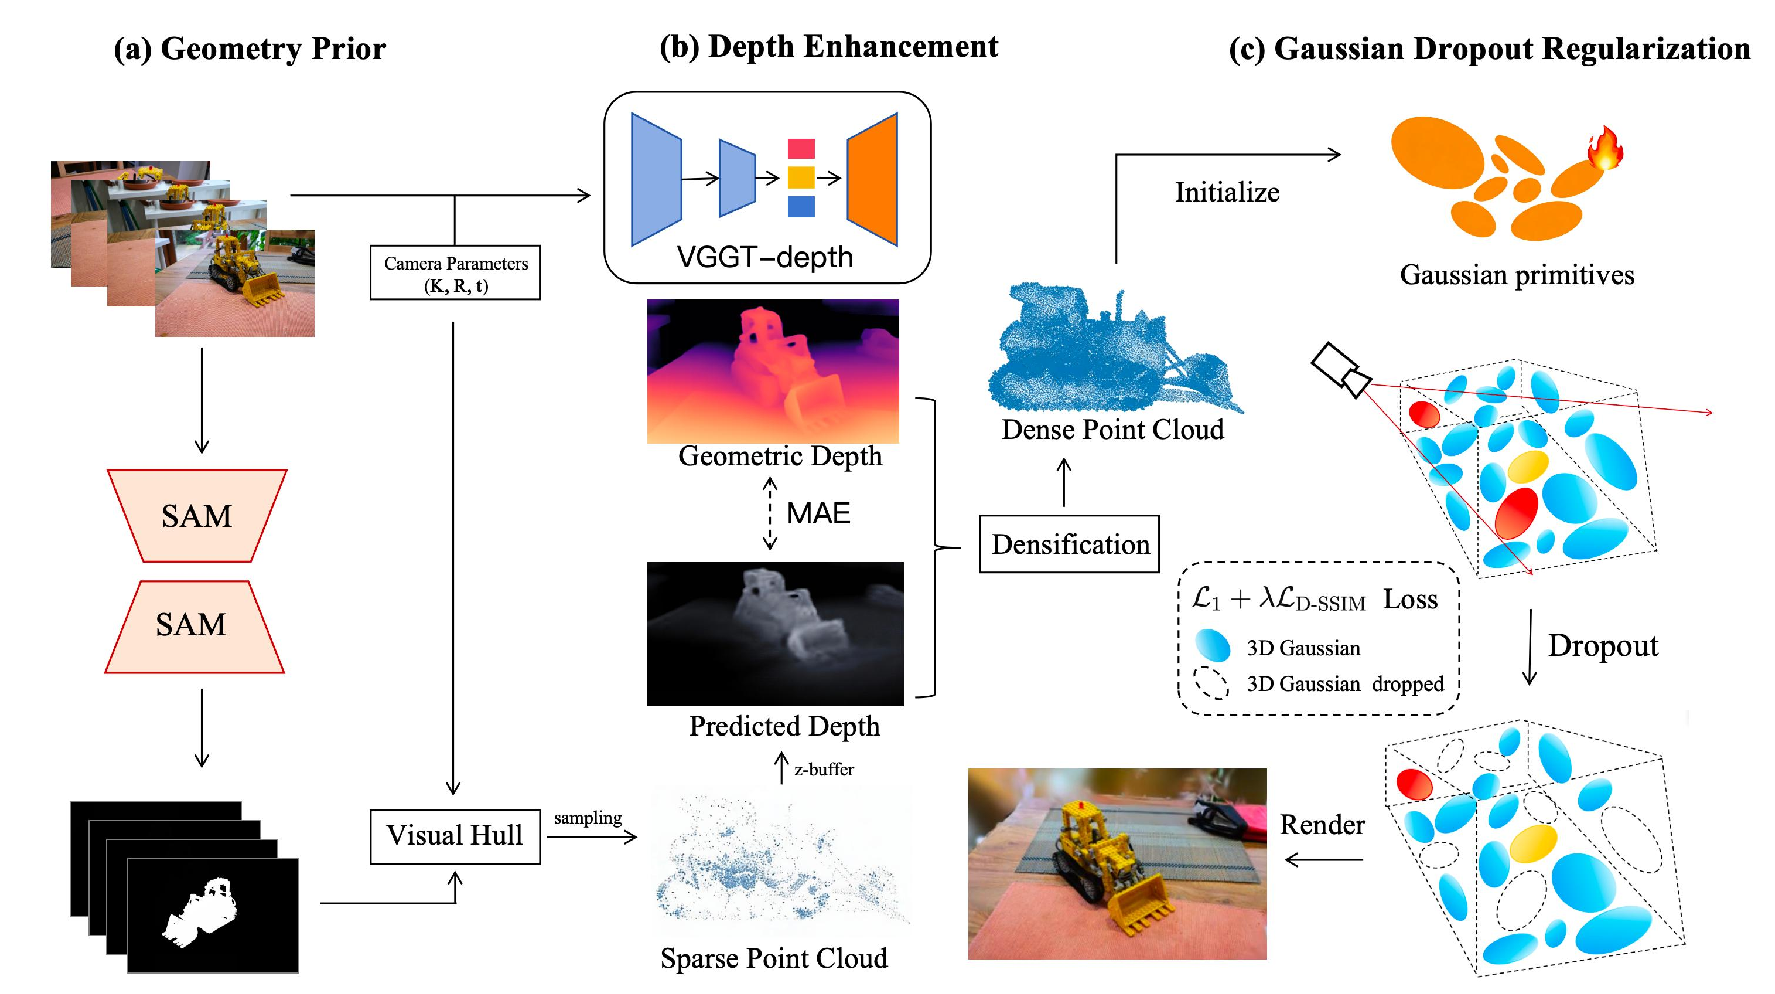
\includegraphics[width=\textwidth]{figures/framework.pdf}
% \caption{Overview of the SynGS pipeline. The third stage applies Dynamic Visibility Regularization (DVR).}
% \label{fig:framework}
% \end{figure}

The pipeline contains three consecutive stages. First, \textbf{Visual Hull Initialization} constructs a coarse geometric prior from multi-view silhouettes and generates an initial point cloud. Then, \textbf{VGGT / Depth-Guided Densification} exploits cross-view depth priors to supplement missing geometry and produce a depth-enhanced point cloud for Gaussian initialization. Finally, \textbf{Dynamic Visibility Regularization (DVR)} is applied during 3DGS optimization to rebalance supervision under sparse visibility and reduce overfitting artifacts. The complete process follows the pipeline:
\begin{equation}
\label{eq:pipeline}
\text{Visual Hull point cloud}
\rightarrow
\text{depth-enhanced point cloud}
\rightarrow
\text{Gaussian initialization}
\rightarrow
\text{DVR-regularized 3DGS optimization}.
\end{equation}

\subsection{Visual Hull Initialization}
\label{sec:visual_hull}

Under sparse views, Structure-from-Motion (SfM)~\cite{Schonberger16_COLMAP} often produces sparse and incomplete point clouds. Weak coverage then destabilizes 3DGS optimization. We construct a Visual Hull prior from sparse multi-view images, camera parameters, and foreground masks, with light mask cleanup at boundaries. With known cameras, silhouettes are back-projected into 3D, and multi-view silhouette consistency defines a coarse geometric envelope of the target~\cite{Laurentini94_VisualHull,Lysykh25_VisualHull}.

Candidate points are retained only when their projections agree with all valid foreground masks, then cleaned by one-time statistical and radius-based outlier filtering~\cite{Balta18_SOR}. The scaffold is stable but coarse: silhouette-based reconstruction cannot fully recover concave regions and fine structures; surface-oriented Gaussian reconstructions similarly indicate that opacity/surface modeling alone still benefits from denser geometric cues~\cite{Guedon24_SuGaR,Yu24_GOF}. Sec.~\ref{sec:depth_densify} supplements the missing geometry before Gaussian initialization.

\subsection{VGGT / Depth-Guided Densification}
\label{sec:depth_densify}

The Visual Hull provides a stable coarse geometric prior, but silhouette constraints alone cannot fully recover concave regions and fine structures. We therefore densify the Visual Hull point cloud with \textbf{VGGT-Depth}: starting from a pre-trained VGGT backbone~\cite{ref30}, we train a depth prior adaptation branch with cross-attention over multi-view tokens and a lightweight fusion head to predict per-view depth maps and confidence estimates under a shared geometric context. As illustrated in Fig.~\ref{fig:vggt_depth}, these adapted multi-view depth priors are used to identify reliable observations, supplement missing geometry, and assist Gaussian attribute initialization. Our remaining design then focuses on reliable depth selection, 3D point supplementation and fusion, and using these cues for Gaussian initialization.

% Placeholder — replace path when the figure is ready
% \begin{figure}[ht]
% \centering
% 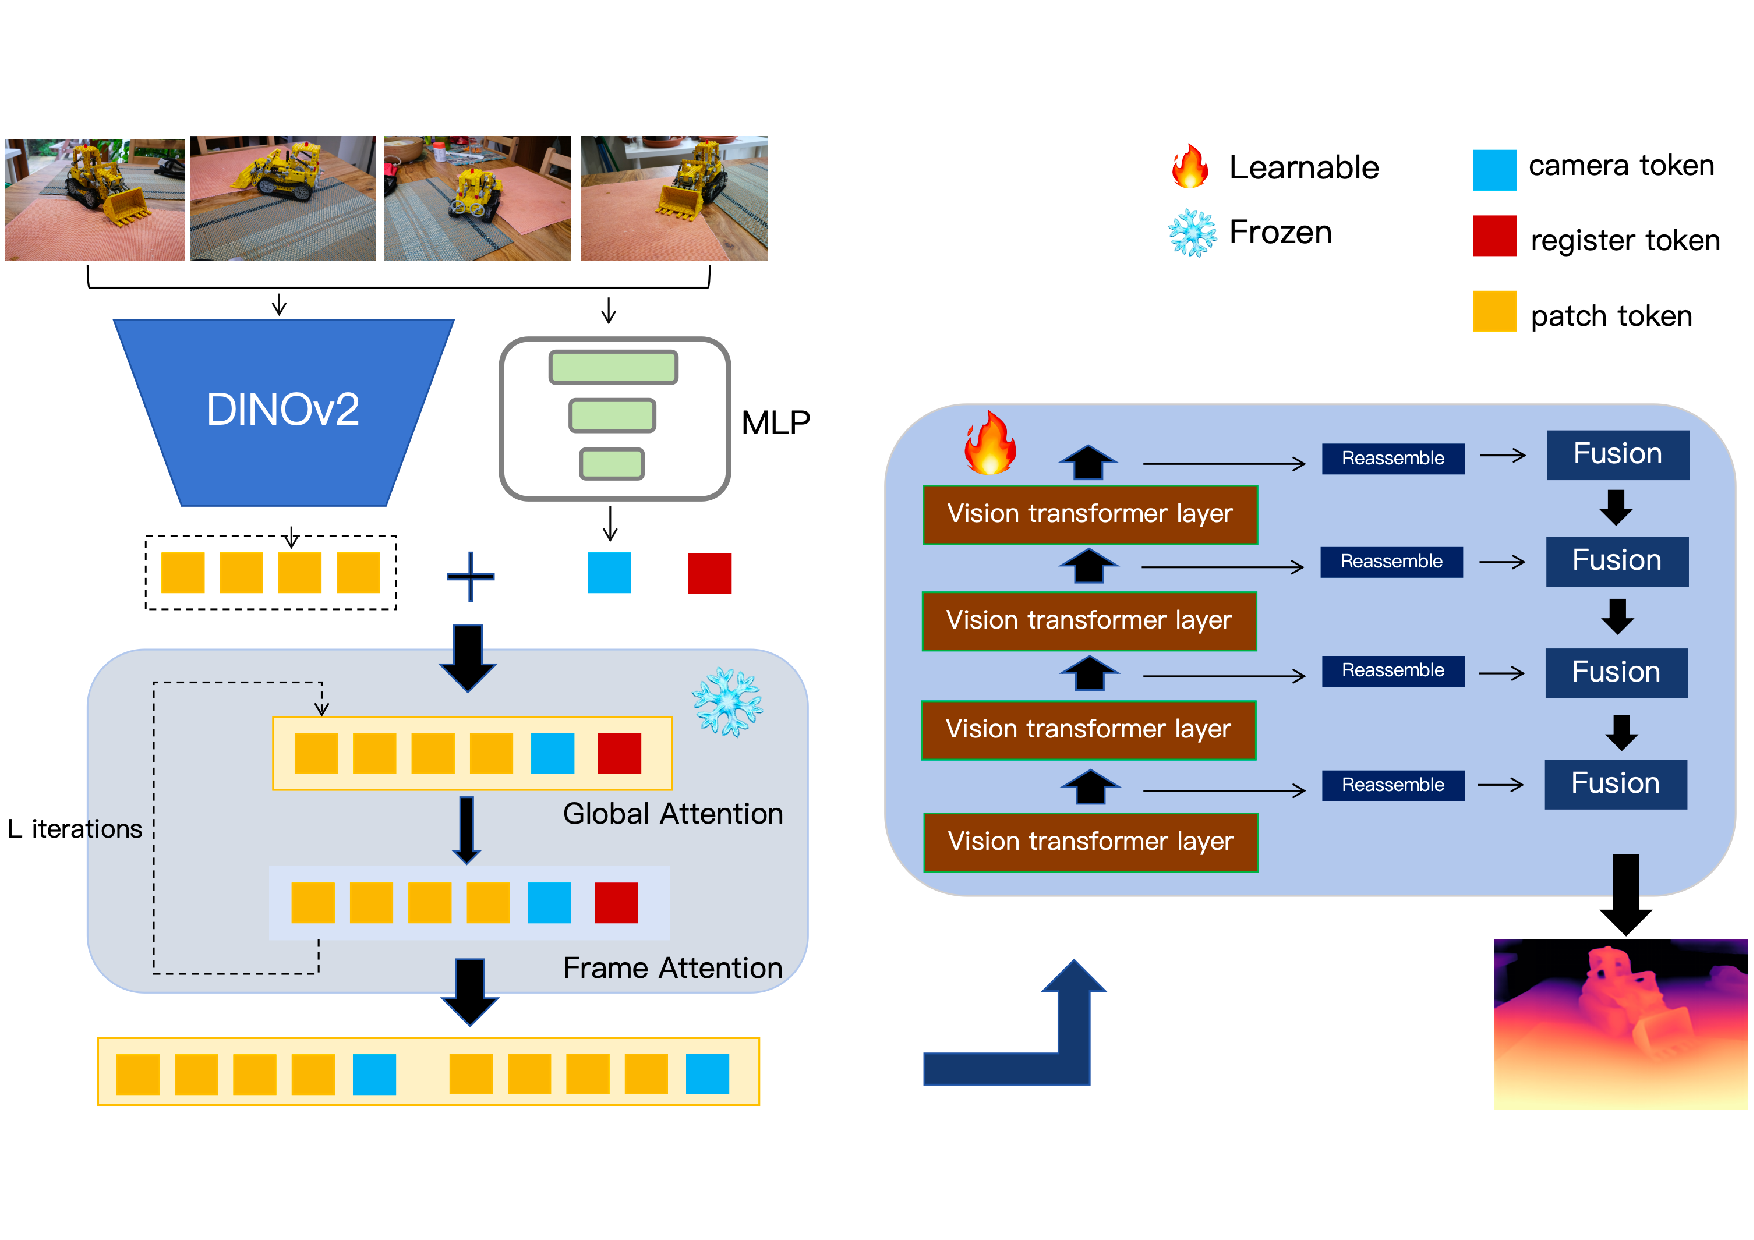
\includegraphics[width=\textwidth]{figures/vggt_depth.pdf}
% \caption{VGGT-Depth prior used for depth-guided point cloud densification.}
% \label{fig:vggt_depth}
% \end{figure}

We use the diagonal length $L$ of the Visual Hull AABB as the scene-scale reference. Before point supplementation, the predicted depth maps are screened at both the view and ray levels. For each view, the masked depth MAE against the dataset ground-truth depth is normalized by the 95th percentile over the validation views to obtain a quality score $q_v$. Views with $q_v<0.4$ are discarded. If fewer than $0.8N$ views remain, depth densification is skipped and the original Visual Hull point cloud is retained. For the selected views, reliable regions are further determined using the VGGT-Depth prediction, its confidence, and depth consistency. We use a depth-adaptive tolerance
\begin{equation}
\label{eq:delta_d}
\Delta(d)=\alpha d+\beta,\qquad
\alpha=0.01,\quad \beta=0.002L,
\end{equation}
and reject low-confidence or depth-inconsistent observations before back-projection.

Point supplementation is performed only along reliable rays. For each point to be supplemented, the top $K=3$ reliable views are selected, and candidate points are sampled around the predicted depth and back-projected into 3D. The supplementary points are merged with the Visual Hull point cloud through two-stage voxel fusion and deduplication, using voxel sizes of $0.01L$ and $0.004L$ for coarse merging and local uniformization, respectively. The resulting densified point cloud provides the geometric input for Gaussian initialization.

Each densified point directly initializes a Gaussian center, while its scale is estimated from the average distance to its $k=8$ nearest neighbors. Multi-view colors are fused using depth-consistency and VGGT confidence weights for appearance initialization. Opacity is initialized from the corresponding cross-view consistency scores and clipped to $[0.2,0.8]$. This process converts the coarse Visual Hull prior into a more complete Gaussian initialization. Sparse-view optimization can still produce uneven supervision across Gaussian primitives with different visibility. We address this issue in the next stage using DVR (Sec.~\ref{sec:dvr}).

\subsection{Dynamic Visibility Regularization}
\label{sec:dvr}

Sparse-view optimization remains strongly visibility-dependent. Distant, occluded, or poorly observed Gaussians appear in fewer views or pixels and receive weaker reconstruction gradients~\cite{Xu25_DropoutGS,Park25_DropGaussian}. Visibility priors have also been explored to regularize sparse-input radiance fields~\cite{Somraj23_ViPNeRF}, and distractor-aware training further highlights sensitivity to unreliable observations~\cite{Sabour24_SpotlessSplats}. Beyond fixed densification heuristics, densification can also be cast as stochastic sampling~\cite{Kheradmand24_3DGSMCMC}, while constraining the Gaussian budget motivates careful control of which primitives participate in rendering~\cite{Fang24_MiniSplatting}. We use DVR via progressive Gaussian dropout.

At iteration $t$, DVR randomly masks a subset of Gaussians for dropout rendering. The dropout ratio grows linearly:
\begin{equation}
\label{eq:dropout_ratio}
r_t=\min\left(r_{\max},\,\gamma\frac{t}{T}\right),
\end{equation}
where $t$ and $T$ are the current and total iterations, $r_{\max}$ is the maximum dropout ratio, and $\gamma=0.1$--$0.2$ controls the growth rate. Early training keeps weak dropout for geometric convergence; later training increases it against sparse-view overfitting.

Used alone, random dropout can induce opacity or scale compensation; we keep a full-render branch as an anchor. Unlike compensated rendering that rescales retained primitives~\cite{Park25_DropGaussian}, the dropout branch is left uncompensated, while the full set is rendered in parallel under the same target. Let $I_{\mathrm{full}}$ and $I_{\mathrm{drop}}$ denote the full and dropout renderings, and $I$ the ground-truth image. We use the standard color loss
\begin{equation}
\label{eq:color_loss}
\mathcal{L}_{\mathrm{color}}(\hat{I},I)
=
(1-\lambda)\,\mathcal{L}_{1}(\hat{I},I)
+
\lambda\,\mathcal{L}_{\mathrm{D\text{-}SSIM}}(\hat{I},I),
\end{equation}
with $\lambda=0.2$~\cite{Kerbl23_3DGS}. The final objective is
\begin{equation}
\label{eq:dvr_loss}
\mathcal{L}
=
\mathcal{L}_{\mathrm{color}}(I_{\mathrm{full}},I)
+
\beta\,\mathcal{L}_{\mathrm{color}}(I_{\mathrm{drop}},I),
\end{equation}
where $\beta=0.5$--$1.0$. Related sparse-view designs further modulate masking with depth and density cues~\cite{Song26_D2GS}, or drop anchors and spherical harmonics~\cite{Fang26_DropAnSH}; DVR instead uses a progressive random schedule with an uncompensated dropout branch.


% Experiments — SPIE section title ALL CAPS; subsections in separate files
\section{EXPERIMENTS}
\label{sec:experiments}

\subsection{Experimental Setup and Datasets}
\label{sec:setup}

We evaluate SynGS on two widely used novel view synthesis benchmarks: Mip-NeRF 360~\cite{Barron22_MipNeRF360} and LLFF 360~\cite{Mildenhall19_LLFF}. All images are downsampled by a factor of 8. Following sparse-view evaluation protocols, Mip-NeRF 360 scenes are tested with 4, 6, and 9 uniformly sampled input views. The reconstruction quality is evaluated using PSNR, SSIM~\cite{Wang04_SSIM}, and LPIPS~\cite{Zhang18_LPIPS}.

We compare against the baselines reported in Tables~\ref{tab:mip360} and~\ref{tab:llff}: RegNeRF~\cite{Niemeyer22_RegNeRF}, SparseNeRF~\cite{Wang23_SparseNeRF}, 3DGS~\cite{Kerbl23_3DGS}, CoR-GS~\cite{Zhang24_CoRGS}, DropGaussian~\cite{Park25_DropGaussian}, and D$^2$GS~\cite{Song26_D2GS}. All methods are evaluated under consistent input settings within each table.

Our implementation follows the standard 3DGS optimization framework. Depth priors are obtained from VGGT-Depth, i.e., a depth prior adaptation branch trained on a pre-trained VGGT backbone. Consistent with Sec.~\ref{sec:depth_densify}, view- and ray-level selection during densification uses dataset ground-truth depth. The model is trained for 30K iterations, with 3DGS initialization optimized for 10K iterations. Floaters are periodically removed during training. Except for the proposed modules, other training configurations follow the vanilla 3DGS settings. Experiments are conducted using PyTorch on an NVIDIA RTX 4090 GPU.

\subsection{Quantitative and Qualitative Results}
\label{sec:results}

% Table 1 — paste full numbers from the manuscript; do not invent values
% Table 1 — data from latex/MipNeRF360数据集/formatting-instructions-latex.tex (unchanged numbers)
\begin{table}[ht!]
\centering
\caption{\label{tab:mip360} Performance comparisons of sparse-view synthesis on Mip-NeRF 360 (4/6/9 views). LPIPS$^{*}$ denotes LPIPS $\times 10^{2}$.}
\setlength{\tabcolsep}{2.8mm}
\renewcommand{\arraystretch}{1.08}
\adjustbox{width=1\linewidth}{%
\begin{tabular}{c l | ccc | ccc | ccc}
\toprule
\multirow{2}{*}{}
  & \multirow{2}{*}{Methods}
  & \multicolumn{3}{c|}{Mip-NeRF 360 (4-view)}
  & \multicolumn{3}{c|}{Mip-NeRF 360 (6-view)}
  & \multicolumn{3}{c}{Mip-NeRF 360 (9-view)} \\
&
  & LPIPS$^{*}$$\downarrow$ & PSNR$\uparrow$ & SSIM$\uparrow$
  & LPIPS$^{*}$$\downarrow$ & PSNR$\uparrow$ & SSIM$\uparrow$
  & LPIPS$^{*}$$\downarrow$ & PSNR$\uparrow$ & SSIM$\uparrow$ \\
\midrule
\sidelabel{2}{NeRF-based}
  & RegNeRF
      & 19.88 & 12.59 & 0.841
      & 20.72 & 13.41 & 0.847
      & 19.70 & 13.68 & 0.852 \\
  & SparseNeRF
      & 17.76 & 12.83 & 0.845
      & 19.74 & 13.42 & 0.861
      & 21.56 & 14.36 & 0.873 \\
\addlinespace[4pt]
\sidelabel{5}{3DGS-based}
  & 3DGS
      &10.80 & 20.31 & 0.899
      &8.38 & 22.12 & 0.913
      &6.42 & 24.29 & 0.930 \\
  & CoR-GS
      &11.76 & 20.45 & 0.856
      &9.28 & 22.57 & 0.901
      &7.04 & 24.73 & 0.926 \\
  & DropGaussian
      &11.57 & 21.76 & 0.837
      &8.61 & 22.98 & 0.895
      &8.02 & 24.10 & 0.915 \\
  & D$^2$GS
      &\cellcolor{color_blue}2.58 &\cellcolor{blue!8}22.35 &\cellcolor{blue!8}0.923
      &\cellcolor{color_blue}2.34 &\cellcolor{blue!8}24.74 &\cellcolor{blue!8}0.937
      &\cellcolor{color_blue}2.11 &\cellcolor{blue!8}27.13 &\cellcolor{blue!8}0.941 \\
  & SynGS (Ours)
      &\cellcolor{blue!8}3.89 &\cellcolor{color_blue}25.91 &\cellcolor{color_blue}0.948
      &\cellcolor{blue!8}3.43 &\cellcolor{color_blue}27.93 &\cellcolor{color_blue}0.953
      &\cellcolor{blue!8}3.02 &\cellcolor{color_blue}29.21 &\cellcolor{color_blue}0.961 \\
\bottomrule
\end{tabular}%
}
\end{table}


\textbf{Mip-NeRF 360.}
Table~\ref{tab:mip360} reports the results on Mip-NeRF 360 under the 4-, 6-, and 9-view settings. SynGS achieves the highest PSNR and SSIM in all three settings, with the largest PSNR advantage appearing in the 4-view case, where it reaches 25.91~dB, 3.56~dB above D$^2$GS~\cite{Song26_D2GS}. The advantage remains clear as the number of input views increases. For LPIPS, however, D$^2$GS obtains lower values across the three settings.

% Table 2 — caption uses ``LLFF 360'' (locked)
% Table 2 — LLFF 360 (locked dataset name). Paste manuscript numbers; do not invent.
% LPIPS* = LPIPS $\times 10^{2}$ throughout this paper.
\begin{table}[t]
\caption{Performance comparisons of sparse-view synthesis on the LLFF 360 dataset (4/6/9 views). LPIPS$^{*}$ denotes LPIPS $\times 10^{2}$.}
\label{tab:llff}
\begin{center}
\begin{tabular}{|l|ccc|ccc|ccc|}
\hline
\rule[-1ex]{0pt}{3.5ex}
 & \multicolumn{3}{c|}{4 views} & \multicolumn{3}{c|}{6 views} & \multicolumn{3}{c|}{9 views} \\
\cline{2-10}
\rule[-1ex]{0pt}{3.5ex}
Method & LPIPS$^{*}$$\downarrow$ & PSNR$\uparrow$ & SSIM$\uparrow$ & LPIPS$^{*}$$\downarrow$ & PSNR$\uparrow$ & SSIM$\uparrow$ & LPIPS$^{*}$$\downarrow$ & PSNR$\uparrow$ & SSIM$\uparrow$ \\
\hline
\rule[-1ex]{0pt}{3.5ex}
% TODO: paste rows from manuscript Table 2 (baselines may differ from Table 1)
\multicolumn{10}{|l|}{\textit{TODO: fill from manuscript Table 2}} \\
\hline
\end{tabular}
\end{center}
\end{table}


\textbf{LLFF 360.}
The LLFF 360 results in Table~\ref{tab:llff} show a similar trend under highly sparse inputs. With four views, SynGS achieves the best PSNR, SSIM, and LPIPS among the compared methods, while under six views it obtains the highest PSNR and SSIM with LPIPS close to the best result. At nine views, the differences become smaller: D$^2$GS~\cite{Song26_D2GS} gives slightly higher PSNR and lower LPIPS, while CoR-GS~\cite{Zhang24_CoRGS} achieves slightly higher SSIM. The clearest advantage appears in the 4- and 6-view settings.

\textbf{Qualitative Results.}
Figure~\ref{fig:qualitative} shows the qualitative comparison under the 4-view setting on Mip-NeRF 360. Compared with the baseline methods, SynGS produces fewer floating artifacts and more complete object boundaries, while preserving finer structures in regions where several competing methods exhibit broken contours or missing details.

\begin{figure*}[t]
\centering
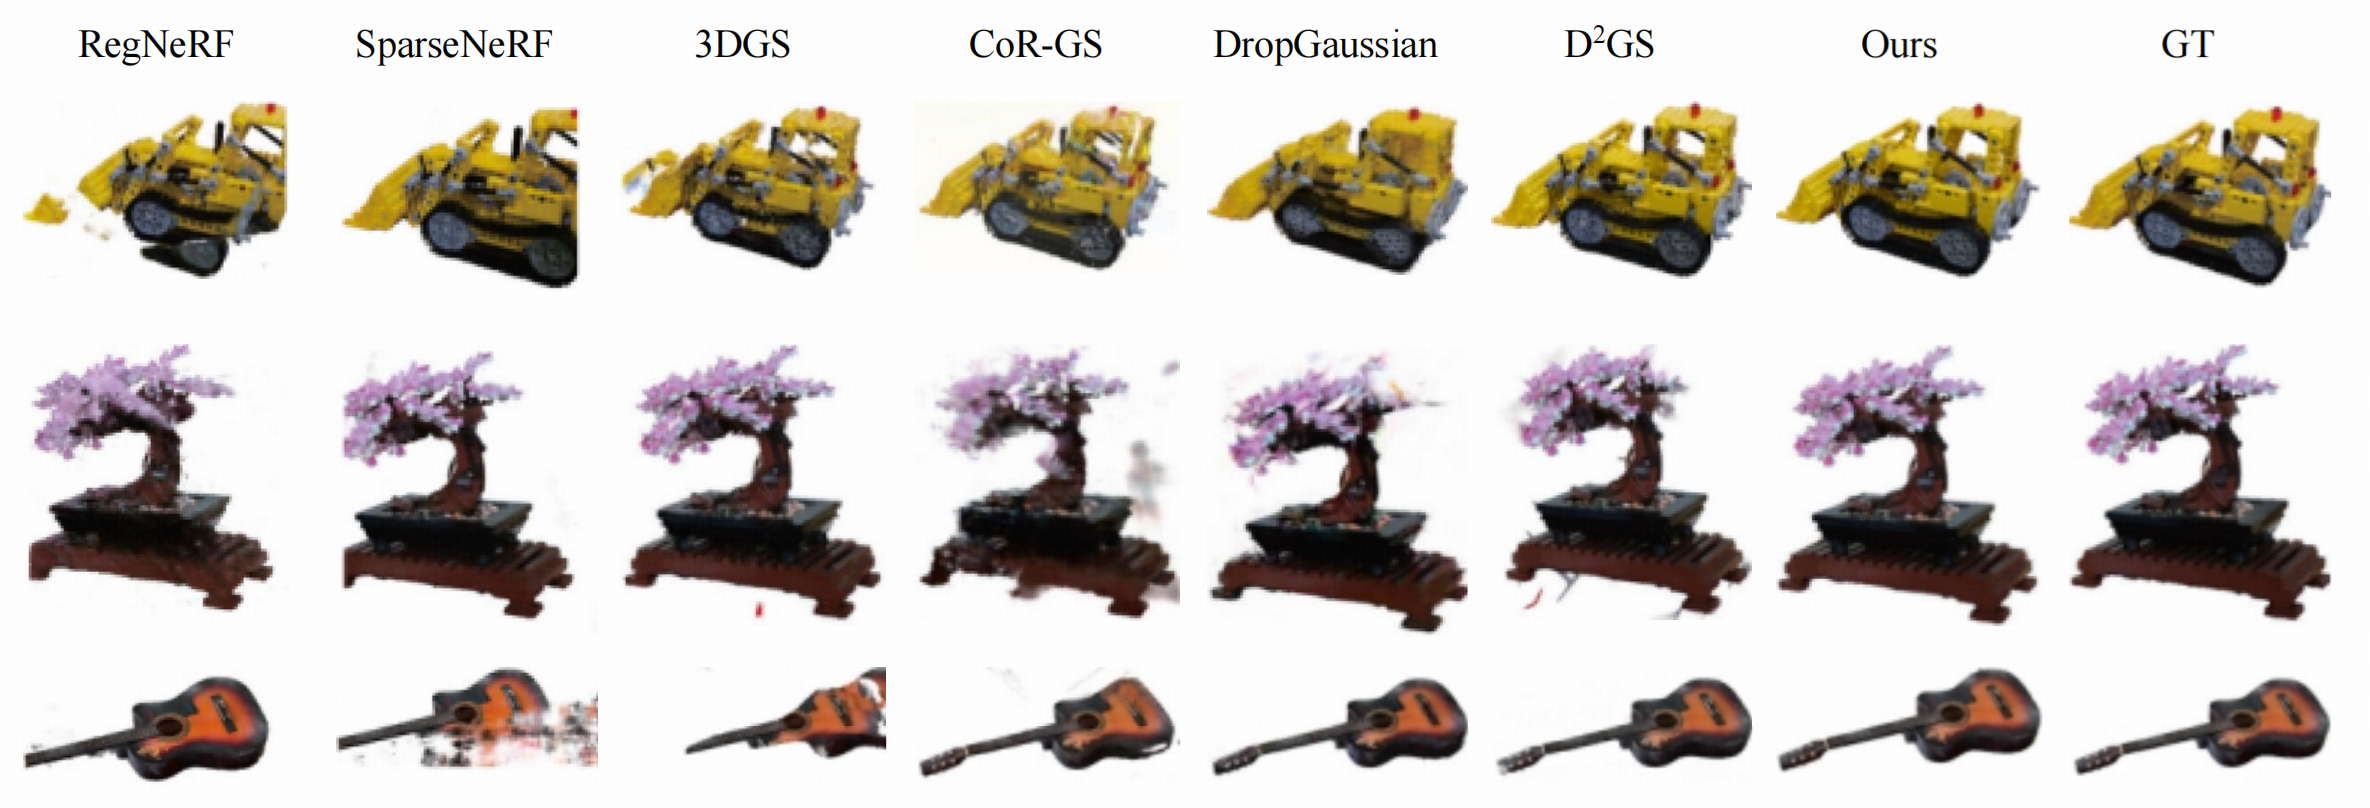
\includegraphics[width=\textwidth]{figures/qualitative.png}
\caption{Qualitative comparison under the 4-view sparse-input setting on Mip-NeRF 360. SynGS produces fewer floating artifacts and more complete structural boundaries than the compared methods.}
\label{fig:qualitative}
\end{figure*}

\subsection{Ablation Study}
\label{sec:ablation}

Table~\ref{tab:ablation} isolates the contributions of the three components under the same training settings.

% Table 3 — Ablation. LPIPS* same scaling as Tables 1--2 ($\times 10^{2}$).
% Column Visibility Balancing* = DVR (footnote).
\begin{table}[t]
\caption{Ablation study of SynGS components. LPIPS$^{*}$ denotes LPIPS $\times 10^{2}$.}
\label{tab:ablation}
\begin{center}
\begin{tabular}{|c|c|c|c|c|c|}
\hline
\rule[-1ex]{0pt}{3.5ex}
Visual Hull Init & Depth Densification & Visibility Balancing$^{*}$ & SSIM$\uparrow$ & PSNR$\uparrow$ & LPIPS$^{*}$$\downarrow$ \\
\hline
\rule[-1ex]{0pt}{3.5ex}
\checkmark &  &  & TODO & 17.51 & TODO \\
\hline
\rule[-1ex]{0pt}{3.5ex}
\checkmark & \checkmark &  & TODO & 24.96 & TODO \\
\hline
\rule[-1ex]{0pt}{3.5ex}
\checkmark & \checkmark & \checkmark & TODO & 26.18 & TODO \\
\hline
\end{tabular}
\end{center}
\vspace{-0.5em}
{\footnotesize $^{*}$Visibility Balancing denotes Dynamic Visibility Regularization (DVR).}
\end{table}


Visual Hull Initialization establishes the geometric baseline at 17.51~dB PSNR. Adding Depth Densification raises PSNR to 24.96~dB, the largest gain in the ablation. Adding DVR further improves the full configuration to 26.18~dB, with gains in SSIM and LPIPS. Across normalized distance intervals, SynGS keeps higher average gradient magnitudes than the baseline, most clearly in the $0.8$--$1.0$ range (about $0.2$ vs.\ $1.2$), indicating stronger supervision on distant, weakly visible primitives.

\clearpage

% Conclusion
\section{CONCLUSION}
\label{sec:conclusion}

% TODO


\bibliography{references}
\bibliographystyle{spiebib}

\end{document}
